This page describes how to use the Poly\-D\-A\-Q G\-U\-I application. This application is written in the Python language, is open source to all who dare try to read and deal with it, and runs on many platforms -- at least Windows$^{\mbox{T\-M}}$ , Mac$^{\mbox{T\-M}}$ , and Linux$^{\mbox{T\-M}}$ .

 
\begin{DoxyImageNoCaption}
  \mbox{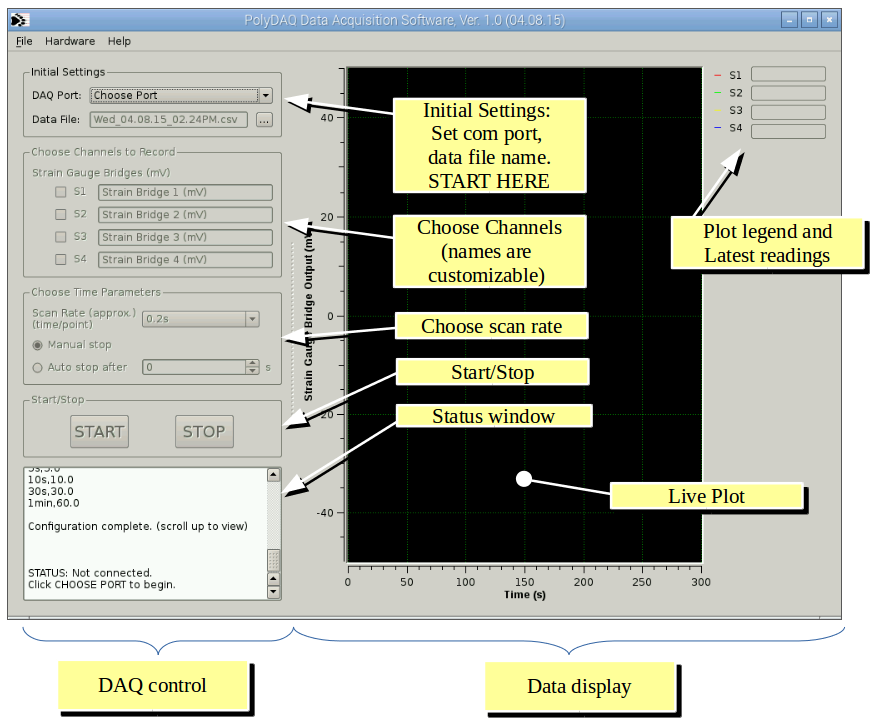
\includegraphics{gui_screenshot_1.png}}
\end{DoxyImageNoCaption}
\hypertarget{pd_py_gui_gui_steps}{}\section{Running the G\-U\-I}\label{pd_py_gui_gui_steps}
To set up and start data collection, follow the following steps\-:
\begin{DoxyEnumerate}
\item {\bfseries Initilize the communication port\-:} Under Initial Settings, click {\ttfamily C\-H\-O\-O\-S\-E} {\ttfamily P\-O\-R\-T} and select the port corresponding to your hardware (Linux\-: usually {\ttfamily /dev/tty\-U\-S\-B0}; Windows$^{\mbox{T\-M}}$ \-: usually {\ttfamily C\-O\-M3} or {\ttfamily C\-O\-M4}, always {\ttfamily C\-O\-M} {\itshape something}.) The status window will indicate that the hardware has been connected and the rest of the interface will be activated. Note\-: If the interface is not activated, check the status window\-: the hardware may not have been connected, or you may not have permission to access the serial port.
\item {\bfseries Change data filename} (optional)\-: The default filename is the date and time you opened the program. This name is unique and will help you identify your file later; however, you may change the file name if you wish.
\item {\bfseries Select channels} and edit channel names\-: Click the boxes coresponding to the channels you wish to record. You may also customize the names of any channel in order to make data labels more meaningful. These names are what will appear in your data file.
\item {\bfseries Balance strain gauge bridges\-:} Strain gauge Wheatstone bridges require balancing prior to start. To run an auto-\/balance on the strain bridges, go to the main menu bar and select {\ttfamily Hardware} -\/$>$ {\ttfamily Auto-\/balance Strain Gauges...}
\item {\bfseries Choose sample rate} and options\-: Select the desired sample rate using the combo box. The sample rate varies slightly due to how the hardware works, but the data file records actual time of measurements, so accurate signal-\/time plots can still be made.

Some sample rates are only achievable if you select fewer channels; this is noted in the combo box.

You can set the D\-A\-Q to record until a specified time, then automatically stop. By default, data is taken until you manually stop it.
\item {\bfseries Start and Stop\-:} These two buttons do exactly what one would expect. Note that after the D\-A\-Q is started, the control panel is inactivated; you cannot change data acquisition parameters while collecting data.
\end{DoxyEnumerate}\hypertarget{pd_py_gui_gui_nav}{}\section{Live Data Navigation}\label{pd_py_gui_gui_nav}
You can explore the data while it is being collected. The latest numerical value for each channel is displayed in the plot legend. The live plot can be navigated in the following ways\-:
\begin{DoxyItemize}
\item {\bfseries y-\/axis controls\-:} Right-\/clicking on the y axis opens a menu where you can
\begin{DoxyItemize}
\item Zoom all y\-: expands the y axis to include the entire range of y values collected {\itshape so} {\itshape far} 
\item Manually set axis limits
\item Turn Auto\-Scale on/off\-: automatically adjust the y-\/axis limits as data is being collected
\end{DoxyItemize}
\item {\bfseries time axis controls\-:} Right-\/clicking the time axis opens a menu where you can
\begin{DoxyItemize}
\item Zoom all time\-: zooms out to display the entire time data has been collected
\item Manually set axis limits
\item Synchronize time axes\-: When more than one plot is displayed, this function updates all plots to the same time range when you pan or zoom in another plot
\end{DoxyItemize}
\item {\bfseries Line display controls\-:} Right-\/clicking on any signal in the plot legend to the right of the plot allows you to
\begin{DoxyItemize}
\item Turn the curve off, to make viewing other channels' data easier. Making the line invisible from the plot does not affect the data being recorded to the data file
\item Change the line properties like color and line thickness
\end{DoxyItemize}
\item {\bfseries Mouse controls\-:} allow panning and zooming
\begin{DoxyItemize}
\item Zoom Window\-: left click-\/and-\/drag draws a rectangle on the plot, then the view zooms in to that rectangle
\item Scroll-\/wheel Zoom\-: using the scroll wheel on your mouse also zooms in or out
\item Pan\-: clicking and dragging on the scroll wheel (middle mouse button) allows you to pan within the plot
\item Undo zoom\-: right-\/clicking anywhere within the plot returns the plot to the previous zoom state 
\end{DoxyItemize}
\end{DoxyItemize}